\documentclass[11pt,letterpaper]{article}
\usepackage[utf8]{inputenc}

%----- Configuración del estilo del documento------%
\usepackage{epsfig,graphicx}
\usepackage[left=2cm,right=2cm,top=1.8cm,bottom=2.3cm]{geometry}
\usepackage{fancyhdr}
\usepackage{lastpage}
\usepackage{url}
\pagestyle{fancy}
\fancyhf{}
\rfoot{\textit{Página \thepage \hspace{1pt} de \pageref{LastPage}}}


%------ Paquetes matemáticos básicos --------%
\usepackage{amsmath}
\usepackage{amssymb}
\usepackage{amsthm}

\usepackage[spanish]{babel}
\usepackage{graphicx}
\usepackage{hyperref}

\usepackage{tabularx}
\usepackage{xcolor}
\usepackage[table]{xcolor}
\usepackage{colortbl}
\usepackage{array, multirow, multicol, tabularx}
\usepackage{tcolorbox}
\newtheorem{theorem}{Theorem}[section]
\newtheorem{corollary}{Corollary}[theorem]
\newtheorem{lemma}[theorem]{Lemma}

%------si-------%
\definecolor{B}{HTML}{FFFFFF}
\definecolor{G}{HTML}{5e5e5e}
\definecolor{R2}{HTML}{d53d40}
\definecolor{A2}{HTML}{034190}
\definecolor{V2}{HTML}{7faa50}
\newcommand{\R}{\mathbb{R}}
\newcommand{\C}{\mathcal{C}}
\newcommand{\N}{\mathbb{N}}
\newcommand{\Z}{\mathbb{Z}}
\newcommand{\Q}{\mathbb{Q}}
\renewcommand{\theenumi}{\Roman{enumi}}
\renewcommand{\labelenumi}{{\theenumi}.}

\begin{document}

%------ Encabezado -------- %

\begin{center}
    \begin{minipage}{3cm}
    	\begin{center}
    		\includegraphics[height=3.4cm]{logo_unam.png}
    	\end{center}
    \end{minipage}\hfill
    \begin{minipage}{10cm}
    	\begin{center}
    	\textbf{\large Universidad Nacional Autónoma de México}\\[0.1cm]
        \textbf{Facultad de Ciencias}\\[0.1cm]
        \textbf{C\'alculo I}\\[0.1cm]
        Lista 2\\[0.1cm]
         El\'ias L\'opez Rivera\\[0.1cm]
        \texttt{ elias.lopezr\,@ciencias.unam.mx }\\[0.1cm]
        Fecha:\,\,11/07/2025
    	\end{center}
    \end{minipage}\hfill
    \begin{minipage}{3cm}
    	\begin{center}
    		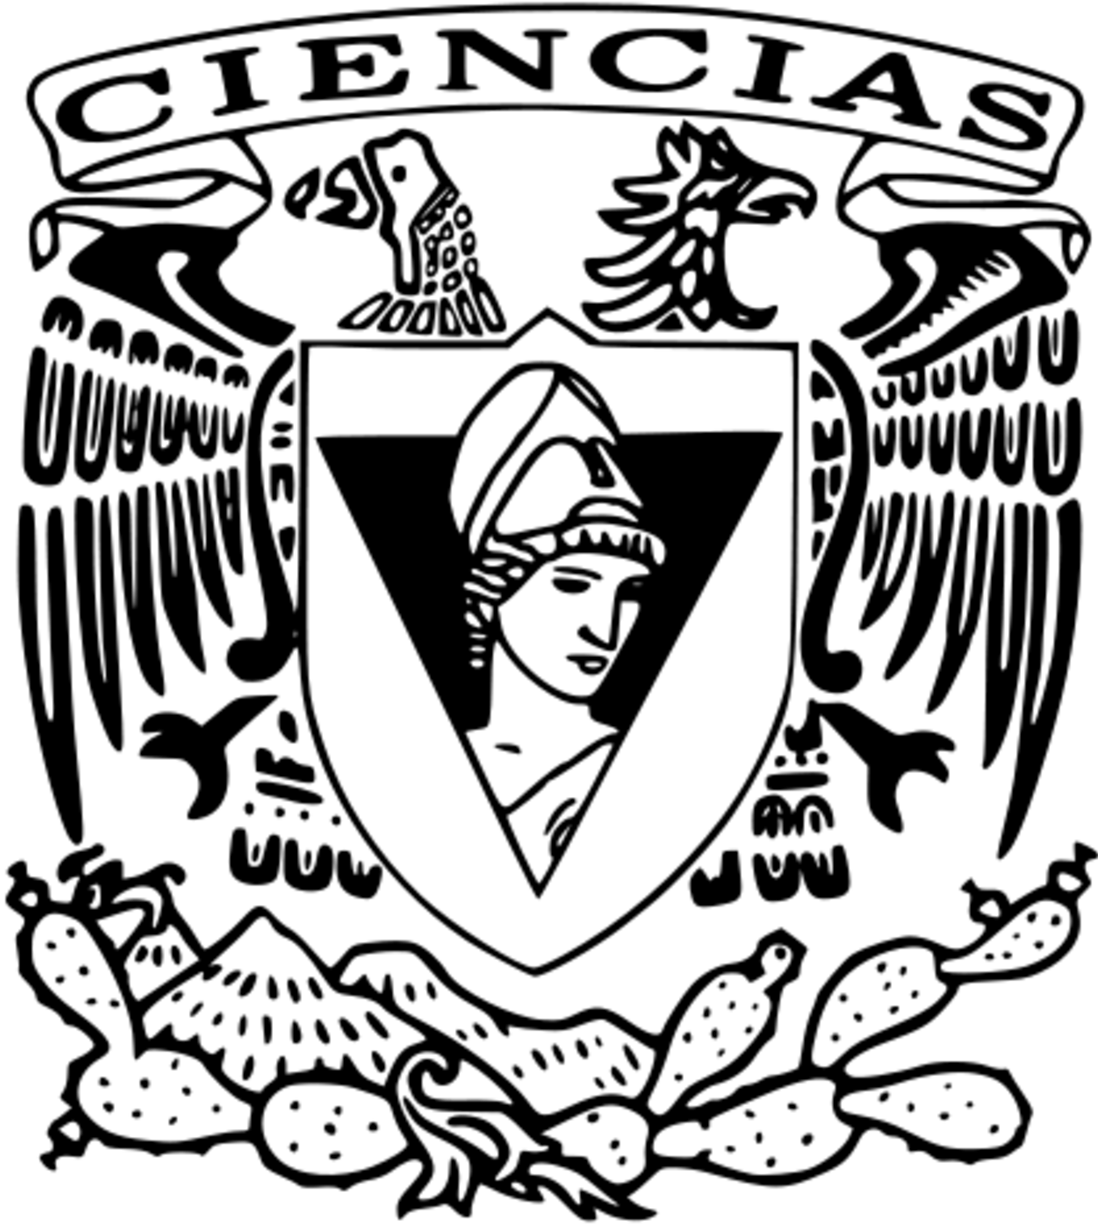
\includegraphics[height=3.4cm]{Logo_FC.png}
    	\end{center}
    \end{minipage}
\end{center}

\rule{17cm}{0.1mm}

%------ Fin de encabezado -------- %
\,\\
\begin{tcolorbox}[
	title = \textcolor{black}{\textcolor{white}{Probelma 36}}]
\textit{Sea $\{f_n\}_{n\in \N}$ la sucesi\'on de Fibonacci
\begin{itemize}
    \item Demuestre que $\sum_{n=1}^{\infty}\,\frac{1}{n^2}$ converge, hint: $\sum_{n=1}^{\infty}\,\frac{1}{n(n+1)}$ converge
    \item Demuestre que $f_{n+2}f_{n}-f^2_{n+1}=(-1)^{n+1}$
    \item Deduzca que:\,\\
    \begin{equation*}
        \left|\frac{f_{n+1}}{f_n}-\frac{f_{n+2}}{f_{n+1}}\right|<\frac{1}{n^2}\,\,\,\,\,\forall\,n>4\,\,\,\,\,n\in \N
    \end{equation*}
    \item Pruebe que:\,\\
    \begin{equation*}
        \lim_{n\rightarrow \infty}\,\frac{f_{n+1}}{f_n}=\frac{1+\sqrt{5}}{2}=\phi
    \end{equation*}
\end{itemize}}
\end{tcolorbox}
\begin{proof}\,\\
    Tenemos que sea $n\in \N$ tal que , entonces $n(n+1)<(n+1)^2$, por tanto $\frac{1}{(n+1)^2}<\frac{1}{n(n+1)}$, por tanto:\,\\
    \,\\
    \begin{equation*}
        1+\sum_{i=2}^{\infty}\,\frac{1}{n}<1+\sum_{i=1}^{\infty}\,\frac{1}{n(n+1)}
    \end{equation*}\,\\
    Por tanto $\sum_{i=1}^{\infty}\,\frac{1}{n^2}$ converge\,\\
    \,\\
    Demostremos que $f_{n+2}f_{n}-f^2_{n+1}=(-1)^{n+1}$, por inducci\'on fuerte:\,\\
    \,\\
    \begin{itemize}
        \item Base de Inducci\'on\,\\
        \begin{equation*}
            f_3f_1-f_2^2=2(1)-1=1^2
        \end{equation*}
        \item Hipotesis de imducci\'on\,\\
        \begin{equation*}
            \exists\,k\in \N : n\leq k\implies f_{n+2}f_{n}-f^2_{n+1}=(-1)^{n+1}
        \end{equation*}
        \item Paso inductivo:\,\\
        \begin{align*}
            f_{k+3}f_{k+1}-f^2_{k+2}=(f_{k+2}+f_{k+1})(f_k+f_{k-1})-(f_{k+1}+f_k)\,\\
            \,\\=f_{k+2}f_{k}-f_{k+1}^2+f_{k+2}f_{k-1}+f_{k+1}f_{k}-2f_{k+1}f_{k}+f_{k+1}f_{k-1}-f_{k}^2\,\\
            \,\\
            \stackrel{\textbf{H.I}}{=}(-1)^{k+1}+f_{k+2}f_{k-1}-f_{k+1}f_k+(-1)^{k}=f_{k+2}(f_{k+1}-f_{k})-f_{k+1}(f_{k+2}-f_{k+1})\,\\
            \,\\
            =-f_{k+2}f_{k}+f_{k+1}^2+f_{k+2}f_{k+1}-f_{k+2}f_{k+1}=-f_{k+2}f_{k}+f_{k+1}^2\stackrel{\textbf{H.I}}{=}(-1)^{k+2}
        \end{align*}
    \end{itemize}
    \,\\
    Ahora demostraremos que $f_n\,f_{n+1}>n^2$ para $n>4$, $n\in\N$, de nuevo por inducc\'on:\,\\
    \begin{itemize}
        \item Base de inducci\'on:
        \begin{equation*}
            f_{5}f_{5+1}=5(8)=40>25=5^2
        \end{equation*}
        \item Hip\'otesis de inducci\'on:
        \begin{equation*}
            \exists\,k\in\N:f_{k}f_{k+1}\geq k^2\,\,\,\,k>4
        \end{equation*}
        \item Paso inductivo:
        \begin{equation*}
            f_{k+1}f_{k+2}=f_{k+1}(f_{k+1}+f_k)>f_{k+1}(f_k+f_k) \stackrel{\textbf{H.I}}{\geq}2k^2
        \end{equation*}\,\\
        Como $k>2$ entonces $k(k-2)>1\implies k^2>2k+1\implies 2k^2>(k+1)^2$, por tanto:\,\\
        \begin{equation*}
             f_{k+1}f_{k+2}>2k^2>(k+1)^2
        \end{equation*}
    \end{itemize}\,\\
    De lo anterior tenemos que:\,\\
    \,\\
    \begin{equation*}
        \left|\frac{f_{n+1}}{f_n}-\frac{f_{n+2}}{f_{n+1}}\right|=\left|\frac{f_{n+1}^2-f_nf_{n+2}}{f_nf_{n+1}}\right|=\left|\frac{(-1)^{n+1}}{f_nf_{n+1}}\right|=\frac{1}{f_nf_{n+1}}<\frac{1}{n^2}
    \end{equation*}\,\\
    \,\\
    Luego tenemos que la serie $\sum_{k\in \N}\,\frac{1}{n^2}$ converge por criterio de la integral, entonces sea $\epsilon>0$ existe $r\in \N$ tal que si $m>k>r$, entonces $\sum_{i=k+1}^m\,\frac{1}{i^2}<\epsilon$, luego tenemos que:\,\\
    \,\\
    \begin{equation*}
        \left|\frac{f_{m+2}}{f_{m+1}}-\frac{f_{k+2}}{f_{k+1}}\right|\leq\left|\frac{f_{m+2}}{f_{m+1}}-\frac{f_{m+1}}{f_{m}}\right|+\left|\frac{f_{m+1}}{f_{m}}-\frac{f_{m}}{f_{m-1}}\right|+\cdots+\left|\frac{f_{k+3}}{f_{k+2}}-\frac{f_{k+2}}{f_{k+1}}\right|<\frac{1}{m^2}+\frac{1}{(m-1)^2}+\cdots+\frac{1}{(k+1)^2}\leq \epsilon
    \end{equation*}\,\\
    Por tanto la sucesi\'on $a_n=\frac{f_{n+1}}{f_n}$ es de Cauchy y es convergente, ahora notemos que:\,\\
    \,\\
    \begin{equation*}
        a_n=\frac{f_{n+1}}{f_n}=\frac{f_n+f_{n-1}}{f_n}=1+\frac{f_{n-1}}{f_n}=1+\frac{1}{a_{n-1}}
    \end{equation*}\,\\
    Por tanto tenemos que $\lambda:=\displaystyle\lim_{n\rightarrow \infty}\,a_n$ cumple que:\,\\
    \,\\
    \begin{equation*}
        \lambda=1+\frac{1}{\lambda}\implies \lambda^2=\lambda+1\implies \lambda^2-\lambda-1=0
    \end{equation*}\,\\
    De donde se sigue que $\lambda=\frac{1+\sqrt{5}}{2}$ o $\lambda=\frac{1-\sqrt{5}}{2}$, como $a_n>0$ para toda $n\in \N$, se conlcuye que \\$\lambda=\frac{1+\sqrt{5}}{2}=\phi$
\end{proof}
\end{document}